\section{Compactness}

    \begin{definition}
    A collection $\mathscr{C}$ of subsets of a space $X$ is said to \textbf{cover} $X$, or to be a \textbf{covering} of $X$, if the union of the elements of $\mathscr{C}$ is equal to $X$. It is called an \textbf{open covering} of $X$ if its elements are open subsets of $X$. 
    \end{definition}

    \begin{definition}
    A space $X$ is said to be \textbf{compact} if every open covering of $X$ contains a finite subcovering (i.e. a finite collection of subcovers) of $X$. It may be better to think of compactness as such: If you can find any infinite open covering of the space, then it is not compact. 
    \end{definition}

    \begin{lemma}
    Let $Y$ be a subspace of $X$. Then $Y$ is compact if and only if every covering of $Y$ by sets open in $X$ contains a finite subcollection covering $Y$. 
    \end{lemma}

  \subsection{Intuition behind Compactness}

    The concept of compactness does not seem intuitive at first glance. The reason why compactness is such an important property for a space to have is because $X$ being compact tells us that we can \textbf{always} analyze the entire $X$ using a \textbf{finite} union of open sets, which can simplify the space greatly. That is, it a measure of finiteness of a space. 

    It is well known that the behavior of finite sets and infinite sets can be different. For example, the four statements below are easily seen to be true whenever $X$ is a finite set, but false whenever $X$ is an infinite set. 
    \begin{enumerate}
        \item (All functions are bounded) If $f: X \longrightarrow \mathbb{R}$ is a real valued function on $X$, then $f$ must be bounded. That is, there exists a finite number $M$ such that $|f(x)| \leq M$ for all $x \in X$. 
        \item (All functions attain a maximum) If $f: X \longrightarrow \mathbb{R}$ is a real-valued function on $X$, then there must exist at least one point $x_0 \in X$ such that $f(x_0) \geq f(x)$ for all $x \in X$. 
        \item (All sequences have constant subsequences) If $(x_\alpha)_{\alpha \in \mathbb{N}}$ is a sequence in $X$, then there must exist a subsequence $x_{\beta_1}, x_{\beta_2}, x_{\beta_3}, ...$ which is constant. That is, $x_{\beta_1} = x_{\beta_2} = x_{\beta_3} = \cdot = c$ for some $c \in X$. 
        \item (All covers have finite subcovers) If $V_1, V_2, V_3, \cdot \subset X$ are any collection of sets which cover $X$, then there must exist a finite sub-collection $V_{n_1}, V_{n_2}, ..., V_{n_k}$ of these sets which still cover $X$. 
    \end{enumerate}

    The fact that all functions on a finite set are bounded is an example of a \textbf{local-to-global principle}. Namely, the hypothesis is an assertion of "local" boundedness: it asserts that $|f(x)|$ is bounded for each point $x \in X$ separately (which can depend on $x$). This collection of local boundedness can be extrapolated to global boundedness: that $|f(x)|$ is bounded by a \textbf{single} bound $M$ for all $x \in X$. This local-to-global boundedness is clearly valid when $X$ is finite, but it fails when $X$ is finite. For example, consider the function
    \[id: \mathbb{N} \longrightarrow \mathbb{R}\]
    which is clearly not bounded by any finite element in $\mathbb{R}$. 

    However, given that we endow a metric or a topology on the set $X$, we can actually find some infinite sets that are "almost finite," in the way that they satisfy a modified version of these four assertions, which are created by introducing topological concepts such as continuity, convergence, and openness. One such "almost finite" set is the closed interval $[0,1]$. 
    \begin{enumerate}
        \item (All \textbf{continuous} functions are bounded) If $f: X \longrightarrow \mathbb{R}$ is a real-valued continuous function on $X$, then $f$ must be bounded. (This is another type of local-to-global principle; if a function is stable with respect to local perturbations, then it is stable with respect to global perturbations).
        \item (All \textbf{continuous functions} attain a maximum) If $f: X \longrightarrow \mathbb{R}$ is a real-valued continuous function on $X$, then there exists at least one point $x_0 \in X$ such that $f(x_0) \geq f(x)$ for all $x \in X$. 
        \item (All sequences have convergent subsequences) If $x_1, x_2, ... \in X$ is a sequence of points in $X$, then there must exist a subsequence $x_{n_1}, x_{n_2}, ...$ which is convergent to some limit $c \in X$. (Bolzano-Weierstrass theorem).
        \item (All open covers have finite subcovers) If $V_1, V_2, V_3, ... \subset X$ are any collection of open sets which cover $X$, then there must exist a finite subcollection $V_{n_1}, V_{n_2}, ..., V_{n_k}$ of these sets which still cover $X$. 
    \end{enumerate}

    However, the open interval $(0,1)$ clearly does not satisfy any of these properties. For example, the continuous function 
    \[f: (0,1) \longrightarrow \mathbb{R}, \; f(x) \equiv \frac{1}{1-x}\]
    does not satisfy the boundedness condition, meaning that it does not satisfy the local-to-global principle. That is, $f$ is not stable under local perturbations of $x$. As you can guess by now, these "almost finite" sets that satifies these "weakened" topological conditions are compact sets. 
    \[\begin{tikzcd}
    Compact \;Sets \arrow{r}{satisfies} & Compact \;Conditions \\
    Finite \;Sets \arrow{r}{satisfies} & Finite \;Conditions \arrow{u}{weakened}
    \end{tikzcd}\]

    However, the four properties are not exactly equivalent, so we can define compactness according to the fourth property: that every open cover has a finite subcover. There are other notions of compactness, such as \textbf{sequential compactness}, which is based on the third version: all sequences have convergent subsequences. 

    Compactness if a powerful property of spaces with many applications. One is via appeal to local-to-global principles; one establishes local control on some function or other quantity, and then uses compactness to boost the local control to global control. Another is to locate amaxima or minima of a function. Of course, many spaces of interest are not compact. For instance, the real line $\mathbb{R}$ is not compact because contains sequences such as $1, 2, 3, \cdot$ which are "trying to escape" the real line, and are not leaving behind and convergent subsequences. However, one can recover compactness by adding a few more points to the space, a process known as \textbf{compactification}. We can add one point at either end of the real line, at $+\infty$ and $-\infty$, resulting in the compact \textbf{extended real line}. 


    \begin{example}
    The subset $Y \equiv (0,1) \times (0,1) \subset \mathbb{R}^2$ is not compact. That is, we can choose to cover the subspace by the finite union of open sets. 
    \[[0,1]^2 \subset \bigcup_{k=0}^\infty \Big( \frac{2^k - 1}{2^k}, \frac{2^{k+1} - 1}{2^{k+1}} \Big) \times (0,1)\]
    We show the first three elements of the infinite union that covers the open square.  
    \begin{center}
    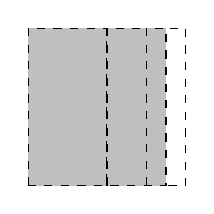
\begin{tikzpicture}[scale=2]
        \draw[dashed] (0,0) rectangle (1,1);
        \draw[dashed, fill=lightgray] (0,0) rectangle (0.5,1);
        \draw[dashed, fill=lightgray] (0.5,0) rectangle (0.75,1);
        \draw[dashed, fill=lightgray] (0.75,0) rectangle (0.875,1);
    \end{tikzpicture}
    \end{center}
    \end{example}

    \begin{theorem}
    Every closed subset of a compact space is compact. 
    \end{theorem}
    \begin{proof}
    This proof is quite trivial. Let $Y$ be a closed subset of compact space $X$. Given a covering $\mathcal{C}$ of $Y$ by sets open in $X$, let us form an open covering $\mathscr{B}$ of $X$ by adjoining to $\mathcal{C}$ the single open set $X \setminus Y$. Then, we an see that both $\mathscr{B}$ and $\mathcal{C} \cup (X \setminus Y)$ covers $X$. 
    \[\mathscr{B} = \mathcal{C} \cup (X \setminus Y)\]
    Since $\mathscr{B}$ is finite, the right hand side must also be expressible as a finite union. Looking through $\mathscr{B}$, we can throw away all the open sets that are entirely in $X \setminus Y$. What remains is a finite covering of $Y$. 
    \end{proof}

    \begin{theorem}
    Every compact subset of a Hausdorff space is closed. 
    \end{theorem}
    \begin{proof}
    Let $Y$ be a compact subset of the Hausdorff Space $X$. We claim that $X \setminus Y$ is open. Let $x \in X \setminus Y$. Then, for each point $y_i \in Y$, we can choose disjoint neighborhoods $U_i$ of $x$ and $V_i$ of $y_i$ (using the Hausdorff condition). The collection 
    \[\{V_i \; | \; y_i \in Y\}\]
    is an open covering $Y$. Since $Y$ is compact, there must exist a finite number of open sets $V_1, V_2, ..., V_n$ covering $Y$. Therefore, 
    \[\bigcup_{i=1}^n V_i\]
    contains $Y$ and is disjoint from the intersection of open neighborhoods of $x$
    \[U \equiv \bigcap_{i=1}^n U_i\]
    Therfore, $U$ is an open neighborhood of $x_0$, disjoint from $Y \implies X \setminus Y$ is open $\implies Y$ is closed.
    \end{proof}

    This results gives the following lemma. 

    \begin{lemma}
    If $Y$ is a compact subset of a Hausdorff space $X$ and $x_0$ is not in $Y$, then there exist disjoint open sets $U$ and $V$ of $X$ containing $x_0$ and $Y$, respectively. 
    \end{lemma}

    \begin{center}
    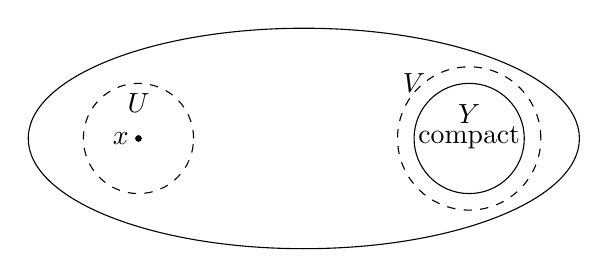
\begin{tikzpicture}[scale=0.7]
        \draw (0,0) ellipse (5 and 2);
        \draw[dashed] (-3,0) circle (1);
        \draw[fill] (-3,0) circle (0.05);
        \node[left] at (-3,0) {$x$};
        \draw (3,0) circle (1); 
        \node[below] at (3,0.8){$Y$};
        \node[below] at (3, 0.4){compact};
        \node[above] at (-3,0.3) {$U$};
        \draw[dashed] (3,0) circle (1.3); 
        \node at (2,1) {$V$};
    \end{tikzpicture}
    \end{center}

    \begin{theorem}
    The image of a compact space under a continuous map is compact.
    \end{theorem}
    \begin{proof}
    Let $f: X \longrightarrow Y$ be continuous, and let $X$ be compact. Let $\mathcal{C}$ be a covering of the set $f(X)$ by sets open in $Y$. Then, the preimage of these sets is the collection
    \[\{f^{-1}(\mathcal{A}) \; | \; \mathcal{A} \in \mathcal{C}\}\]
    which clearly covers $X$. But since $X$ is compact, a finite number of them, say
    \[f^{-1} (\mathcal{A}_1), f^{-1} (\mathcal{A}_2), ..., f^{-1} (\mathcal{A}_n)\]
    covers $X \implies \mathcal{A}_1, \mathcal{A}_2, ..., \mathcal{A}_n$ covers $f(X)$. 
    \end{proof}

    \begin{theorem}
    Let $f: X \longrightarrow Y$ be a bijective continuous function. If $X$ is compact and $Y$ is Hausdorff, then $f$ is a homeomorphism. 
    \end{theorem}
    \begin{proof}
    It suffices to prove that $f$ is an open or closed mapping. We shall show that $f$ is the latter. Let $U$ be closed in $X$. By the previous theorems, $U$ is compact $\implies f(U)$ is compact in Hausdorff $Y \implies f(U)$ is closed. Therefore, $f$ is closed. 
    \end{proof}

    We now introduce a useful lemma that will come around in many future cases. 

    \begin{lemma}[Tube Lemma]
    Consider the product space $X \times Y$, where $Y$ is compact. If $N$ is an open set $X \times Y$ containing the slice $x_0 \times Y$ of $X \times Y$, then $N$ contains some tube $W \times Y$ about $x_0 \times Y$, where $W$ is a neighborhood of $x_0$ in $X$. 
    \end{lemma}
    \begin{center}
    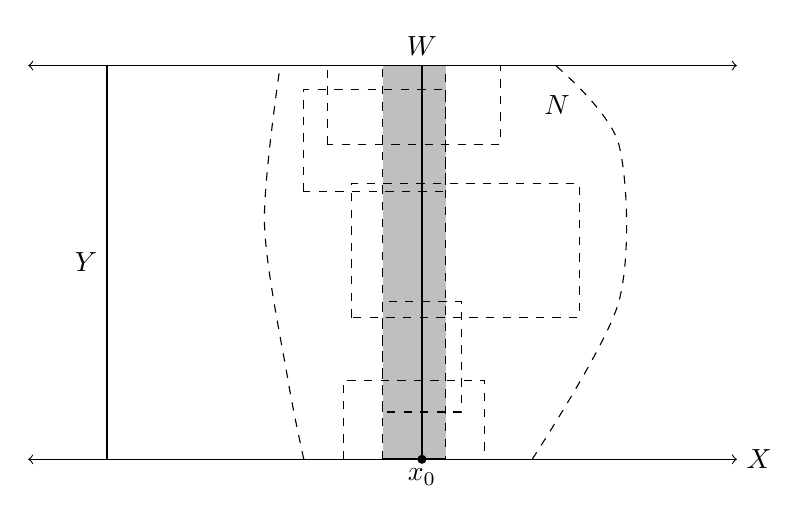
\begin{tikzpicture}
        \draw[dashed, fill=lightgray] (3.5,0) rectangle (4.3,5);
        \draw (0,0)--(0,5);
        \draw[<->] (-1,0)--(8,0);
        \node[right] at (8,0) {$X$};
        \node[left] at (0,2.5) {$Y$};
        \draw[<->] (-1,5)--(8,5);
        \draw[thick] (4,0)--(4,5);
        \draw[dashed] (3,0) rectangle (4.8,1);
        \draw[dashed] (3.5,0.6) rectangle (4.5,2);
        \draw[dashed] (3.1,1.8) rectangle (6,3.5);
        \draw[dashed] (2.5,3.4) rectangle (4.3,4.7);
        \draw[dashed] (2.8,4) rectangle (5, 5);
        \draw[thick] (3.5,0)--(4.3,0);
        \node[above] at (4,5) {$W$};
        \node[below] at (4,0) {$x_0$};
        \draw[fill] (4,0) circle (0.05);
        \draw[dashed] plot [smooth] coordinates {(2.5,0) (2.3, 1) (2,3) (2.2,5)};
        \draw[dashed] plot [smooth] coordinates {(5.4,0) (6.5,2) (6.5,4) (5.7,5)};
        \node[left] at (6,4.5) {$N$};
    \end{tikzpicture}
    \end{center}
    \begin{proof}
    Let us cover $x_0 \times Y$ by basis elements $U \times V$ (for the topology of $X \times Y$) lying in $N$. The space $x_0$ is compact since it is homeomorphic to $Y \implies$ we can cover $x_0 \times Y$ by finitely such basis elements
    \[U_1 \times V_1, U_2 \times V_2, ..., U_n \times V_n\]
    Without loss of generality, we can assume that each $U_i \times V_i$ has a nontrivial intersection with $x_0 \times Y$, since otherwise, it would be superfluous. Now, we define the intersection of all the open neighborhoods of $x_0$ in $X$ of the basis elements $U_i \times V_i$. That is, let
    \[W \equiv \bigcup_{i=1}^n U_i\]
    As an intersection of open sets, $W$ is also open containing $x_0$. With this well-defined tube $W \times Y$, we claim that it is entirely contained within $N$. That is, given a point $x \times y \in W \times Y$, consider the corresponding point $x_0 \times y$ that is the image of the projection of $x\times y$ onto $x_0 \times Y$. Clearly, $x_0 \times y$ belongs to some $U_k \times V_k$ (for some $k$) $\implies y \in V_k$. Since $x \in W$, $x$ is clearly in $U_k$, meaning that $x \times y \in U_k \times V_k \subset N$, as desired. 
    \end{proof}

    \begin{theorem}
    The product of finitely many compact spaces is compact. 
    \end{theorem}
    \begin{proof}
    Using induction, it suffices to prove that the product of 2 compact spaces is compact. Let $X$ and $Y$ be compact spaces. By the tube lemma, for each $x \in X$, there exists a neighborhood $W_x$ of $x$ such that the tube $W_x \times Y$ can be covered with finitely (by compactness of $Y$) many open sets in $X \times Y$. The collection of all neighborhoods $W_x$ is an open covering of $X$. By compactness of $X$, there exists a finite subcollection
    \[W_1, W_2, ..., W_k\]
    covering $X$. The finite union of the tubes 
    \[\bigcup_{i=1}^k W_i \times Y\]
    clearly covers $X \times Y$, meaning that $X \times Y$ is compact. 
    \end{proof}

    \begin{definition}
    A collection $\mathcal{C}$ of subsets of $X$ is said to satisfy the \textbf{finite intersection condition} if for every finite subcollection 
    \[\{\mathcal{C}_1, \mathcal{C}_2, ..., \mathcal{C}_n\}\]
    of $\mathcal{C}$, the intersection
    \[\bigcap_{i=1}^n \mathcal{C}_i\]
    is nonempty. 
    \end{definition}

    Clearly, the empty sets cannot below to any collection with the finite intersection property. Additionally, the condition is trivially satisfied if the intersection over the entire collection is non-empty or if the collection is nested. However, here is one example that does satisfy the finite intersection condition. 

    \begin{example}
    Let $X = (0,1)$ and for each positive integer $i$, $X_i$ is the set of elements of $X$ having a decimal expansion with digit $0$ in the $i$th decimal place. Then, any finite intersection of $X_i$'s is nonempty, but the intersection of all $X_i$ for $i \in \mathbb{N}$ is empty, since no element of $(0,1)$ has all zero digits. 
    \end{example}

    Here is an analogous example to the previous one. 
    \begin{example}
    In the space $\mathbb{R}$, let us define $C_i \equiv \mathbb{R} \setminus \{i\}$. That is, $C_i$ is $\mathbb{R}$ missing a point at $i$. Then, the collection of all $C_i$'s does satisfy the finite intersection condition. We show below the finite intersection of the five subsets $C_0, C_1, C_2, C_3, C_4$. 
    \begin{center}
    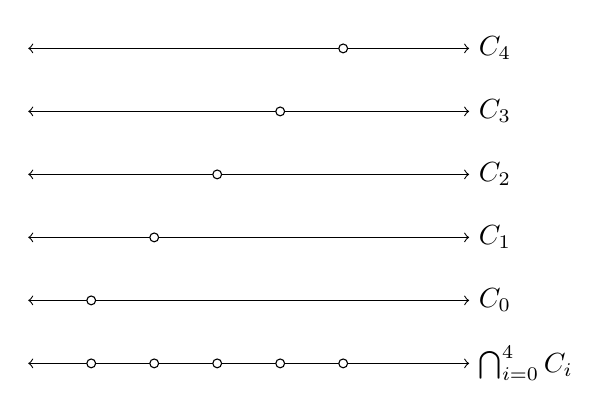
\begin{tikzpicture}[scale=0.8]
        \draw[<->] (-1,0)--(6,0);
        \draw[<->] (-1,1)--(6,1);
        \draw[<->] (-1,2)--(6,2);
        \draw[<->] (-1,3)--(6,3);
        \draw[<->] (-1,4)--(6,4);
        \draw[<->] (-1,-1)--(6,-1);
        \draw[fill=white] (0,0) circle (0.07); 
        \draw[fill=white] (1,1) circle (0.07); 
        \draw[fill=white] (2,2) circle (0.07); 
        \draw[fill=white] (3,3) circle (0.07); 
        \draw[fill=white] (4,4) circle (0.07); 
        \draw[fill=white] (0,-1) circle (0.07); 
        \draw[fill=white] (1,-1) circle (0.07); 
        \draw[fill=white] (2,-1) circle (0.07); 
        \draw[fill=white] (3,-1) circle (0.07); 
        \draw[fill=white] (4,-1) circle (0.07); 
        \node[right] at (6,-1) {$\bigcap_{i=0}^4 C_i$};
        \node[right] at (6,0) {$C_0$};
        \node[right] at (6,1) {$C_1$};
        \node[right] at (6,2) {$C_2$};
        \node[right] at (6,3) {$C_3$};
        \node[right] at (6,4) {$C_4$};
    \end{tikzpicture}
    \end{center}
    \end{example}


    \begin{theorem}
    Let $X$ be a topological space. Then $x$ is compact if and only if for any collection $\mathcal{C}$ of closed sets in $X$ satisfying the finite intersection condition, the intersection 
    \[\bigcap_{C \in \mathcal{C}} C\]
    of all the elements of $\mathcal{C}$ is nonempty. 
    \end{theorem}
    \begin{proof}
    Given a collection $S$ fo subets of $X$, let 
    \[\mathcal{C} \equiv \{X \setminus A \; | \; A \in S\}\]
    be the collection of their complements. Then, the following statements hold 
    \begin{enumerate}
        \item $S$ is a collection of open sets if and only if $\mathcal{C}$ is a collection of closed sets. 
        \item The collection $S$ covers $X$ if and only if the intersection 
        \[\bigcap_{C \in \mathcal{C}} C\]
        of all the elements of $\mathcal{C}$ is empty. 
        \item The finite subcollection $\{A_1, A_2, ..., A_n\}$ of $S$ covers $X$ if and only if the intersection of the corresponding elements $C_i \equiv X \setminus A$ of $\mathcal{C}$ is empty. 
    \end{enumerate}
    Clearly, (1) is trivial, and (2) and (3) follows from DeMorgan's Law. 
    \[X \setminus \bigcup_{\alpha \in J} A_\alpha = \bigcap_{\alpha \in J} (X \setminus A_\alpha)\]
    Using statement 3, the existence of a finite collection of closed sets $C$ in $X$ satisfying the finite intersection condition is equivalent to its complements (which are open sets) covering $X$, which is precisely the definition of compactness. 
    \end{proof}

    Clearly, the previous example in the real line $\mathbb{R}$ shows that $\mathbb{R}$ is indeed not compact. 

    \begin{corollary}
    The space $X$ is compact if and only if every collection $\mathscr{C}$ of subsets of $X$ satisfying the finite intersection condition, the intersection 
    \[\bigcap_{A \in \mathscr{C}} \bar{A}\]
    of their closures is nonempty. 
    \end{corollary}

  \subsection{Compact Sets of the Real Line}

    In order to construct new compact spaces from old ones, we must prove compactness for a number of fundamental spaces. The real number line is a good starting point, and in order to prove that every closed interval in $\mathbb{R}$ is compact, we only need the following theorem. 

    \begin{theorem}
    Let $X$ be a simply ordered set having the least upper bound property (That is, every nonempty subset of $X$ with an upper bound has a least upper bound). Then, in the order topology, every closed interval in $X$ is compact. 
    \end{theorem}

    \begin{corollary}
    Every closed interval in $\mathbb{R}$ is compact. 
    \end{corollary}

    \begin{theorem}[Heine-Borel Theorem]
    A subset $A$ of $\mathbb{R}^n$ is compact if and only if it is closed and bounded in the Euclidean metric $d$ or the square metric $p$. 
    \end{theorem}

    \begin{example}
    The unit sphere $S^{n-1}$ and the closed ball $B^n$ in $\mathbb{R}^n$ are compact since they are closed and bounded. The set
    \[A \equiv \{(x, \frac{1}{x}) \; | \; 0 < x \leq 1\}\]
    is closed in $\mathbb{R}^2$, but is not compact since it is not bounded. The set 
    \[S \equiv \{(x, \sin{\frac{1}{x}}) \; | \; 0<x\leq 1\}\]
    is bounded in $\mathbb{R}^2$, but it is not compact since it is not closed. 
    \end{example}

    \begin{theorem}[Maximum, Minimum Value Theorem]
    Let $f: X \longrightarrow Y$ be continuous, where $Y$ is an ordered set in the order topology. If $X$ is compact, then there exists points $c$ and $d$ in $X$ such that $f(c) \leq f(x) \leq f(d)$ for every $x \in X$. That is, $f$ has a maximum and a minimum at the values $d$ and $c$, respectively. 
    \end{theorem}

  \subsection{Limit Point Compactness}

    We now state different, weaker types of compactness. 

    \begin{definition}
    A space $X$ is said to be \textbf{sequentially compact} if every sequence of points in $X$ has a subsequence that converges to a point $x \in X$. 
    \end{definition}

    \begin{definition}
    A space $X$ is said to be \textbf{countably compact} if every countably open cover has a finite subcover. 
    \end{definition}

    \begin{definition}
    A space $X$ is said to be \textbf{limit point compact} if every infinite subset of $X$ has a limit point. 
    \end{definition}

    \begin{theorem}
    Compactness $\implies$ limit point compactness.  
    \end{theorem}

    \begin{lemma}[Lebesgue Number Lemma]
    Let $\mathscr{C}$ be an open covering of the metric space $(X, d)$. If $X$ is compact, then there is a $\delta > 0$ such that for each subset of $X$ having diameter than $\delta$, there exists an element of $\mathscr{C}$ containing it. This number $\delta$ is called a \textbf{Lebesgue number} for the covering $\mathscr{C}$. 
    \end{lemma}

    Another theorem of calculus, suitably generalized to topological spaces, is stated. 
    \begin{theorem}[Uniform Continuity Theorem]
    Let $f: X \longrightarrow Y$ be a continuous map of the compact metric space $(X,d_X)$ to the metric space $(Y, d_Y$. Then, $f$ is uniformly continuous. That is, given $\epsilon > 0$, there exists a $\delta > 0$ such that for any two points $x_1, x_2 \in X$, 
    \[d_X (x_1, x_2) < \delta \implies d_Y \big( f(x_1), f(x_2)\big) < \epsilon\]
    \end{theorem}

    \begin{theorem}
    Let $(X, \mathscr{T})$ be a metrizable space. Then the following are equivalent: 
    \begin{enumerate}
        \item $X$ is compact. 
        \item $X$ is limit point compact. 
        \item $X$ is sequentially compact. 
        \item $X$ is countably compact. 
    \end{enumerate}
    \end{theorem}

  \subsection{Local Compactness}

    \begin{definition}
    A space $X$ is said to be \textbf{locally compact} at $x$ if there is some compact subset $C$ of $X$ that contains a neighborhood of $x$. If $X$ is locally compact at each of its points, $X$ is simply to be \textbf{locally compact}. 
    \end{definition}

    \begin{example}
    The real line $\mathbb{R}$ is locally compact since any point $x \in \mathbb{R}$ lies within a certain closed interval $[a,b]$, which is compact. The subspace $\mathbb{Q}$ is not locally compact. 
    \end{example}

    Two of the most well-behaved classes of spcaes to deal with are metrizable spaces and compact Hausdorff spaces. If a given space is not one of these types, the next best thing one can hope for is that it is a subspace of one of these spaces. Clearly, a subspace of a metrizable space is itself metrizable, so one does not get any new spaces this way. However, a subspace of a compact Hausdorff space need not be compact. This leads to the question: Under what conditions is a space homeomorphic to a subspace of a compact Hausdorff space? 

    \begin{definition}
    Let $X$ be a locally compact Hausdorff space. Take some object outside $X$, denoted by the symbol $\infty$, and adjoin it to $X$, forming the set
    \[Y = X \cup \{\infty\}\]
    Topologize $Y$ by defining the collection of open sets in $Y$ to be the sets of the following types:
    \begin{enumerate}
        \item $U$, where $U$ is an open subset of $X$. 
        \item $Y \setminus C$, where $C$ is a compact subset of $X$.
    \end{enumerate}
    Then, this space $Y$ is called the \textbf{one-point compactification of $X$}. This is in some sense the minimal compactification of $X$. 
    \end{definition}
    We briefly show that this set of open sets on $Y$ is indeed a topology. First, $\emptyset$ is of type 1 and $Y$ itself is of type 2. Given $U_i$ of type 1 and $Y \setminus C_i$ of type 2, we have the intersections of two sets
    \begin{align*}
        &U_1 \cap U_2 & \text{ is type 1} \\
        &(Y \setminus C_1) \cap (Y \setminus C_2) = Y \setminus (C_1 \cup C_2) & \text{ is type 2} \\
        &U_1 \cap (Y \setminus C_1) = U_1 \cap (X \setminus C_1) & \text{ is type 1} \\
    \end{align*}
    along with the arbitrary union of sets
    \begin{align*}
        &\bigcup U_\alpha = U & \text{ is type 1} \\
        &\bigcup (Y \setminus C_\beta) = Y \setminus (\bigcap C_\beta) = Y \setminus C & \text{ is type 2} \\
        &(\bigcup U_\alpha) \cup ( \bigcup (Y \setminus C_\beta)) = U \cup (Y \setminus C) = Y \setminus (C \setminus U) & \text{ is type 2} \\
    \end{align*}
    We now present some properties of one-point compactifications. 

    \begin{theorem}
    Let $X$ be a locally compact Hausdorff space which is not compact, and let $Y$ be a one-point compactification of $X$. Then $Y$ is a compact Hausdorff space. Additionally, since $X \subset Y$ with $Y \setminus X$ consisting of a single point, $\bar{X} = Y$. 
    \end{theorem}

    \begin{example}
    The one-point compactification of the real line $\mathbb{R}$ is homeomorphic to the circle $S^1$. That is, 
    \[\mathbb{R} \cup \{\infty\} \cong S^1\]
    $\mathbb{R} \cup \{\infty\}$ is called the \textbf{extended real number line}. We can see this homeomorphism by visualizing the stereographic projection $p: S^1 \setminus \{s\} \longrightarrow \mathbb{R}$. 

    \begin{center}
    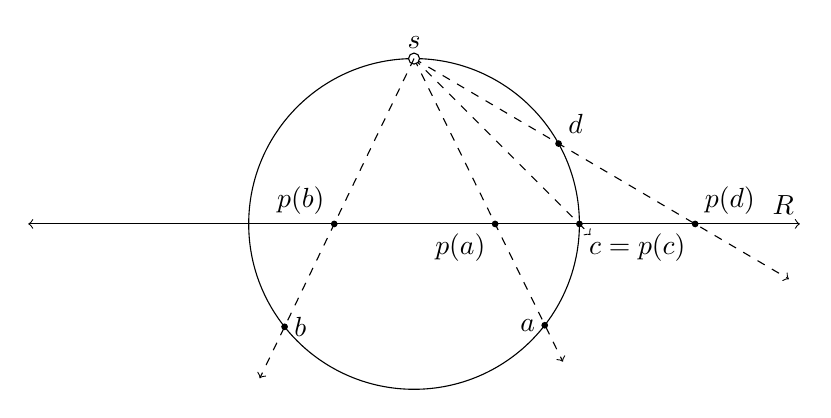
\begin{tikzpicture}[scale=0.7]
      \draw (0,0) circle (3);
      \node[above] at (0,3) {$s$};
      \draw[<->] (-7,0)--(7,0);
      \node[above] at (6.7,0) {$\mathbb{R}$};
      \draw[->, dashed] (0,3)--(3.2,-0.2);
      \draw[->, dashed] (0,3)--(2.7,-2.5);
      \draw[->, dashed] (0,3)--(6.8,-1);
      \draw[fill=white] (0,3) circle (0.1);
      \draw[->, dashed] (0,3)--(-2.8, -2.8);
      \draw[fill] (3,0) circle (0.05);
      \draw[fill] (-2.349,-1.866) circle (0.05);
      \draw[fill] (5.1,0) circle (0.05);
      \draw[fill] (2.622,1.458) circle (0.05);
      \draw[fill] (-1.448,0) circle (0.05);
      \draw[fill] (1.471,0) circle (0.05); 
      \draw[fill] (2.371, -1.838) circle (0.05);
      \node[left] at (2.371, -1.838) {$a$};
      \node[below left] at (1.471,0) {$p(a)$};
      \node[above left] at (-1.448,0) {$p(b)$};
      \node[right] at (-2.349,-1.866) {$b$};
      \node[above right] at (5.1,0) {$p(d)$};
      \node[above right] at (2.622,1.458) {$d$};
      \node[below right] at (3,0) {$c = p(c)$};
    \end{tikzpicture}
    \end{center}
    \end{example}

    \begin{example}
    The one point-compactification of the real plane $\mathbb{R}^2$ is homeomorphic to the 2-sphere $S^2$. That is, 
    \[\mathbb{R}^2 \cup \{\infty\} \cong S^2\]
    We can similarly imagine this homeomorphism using the stereographic projection. 
    \begin{center}
        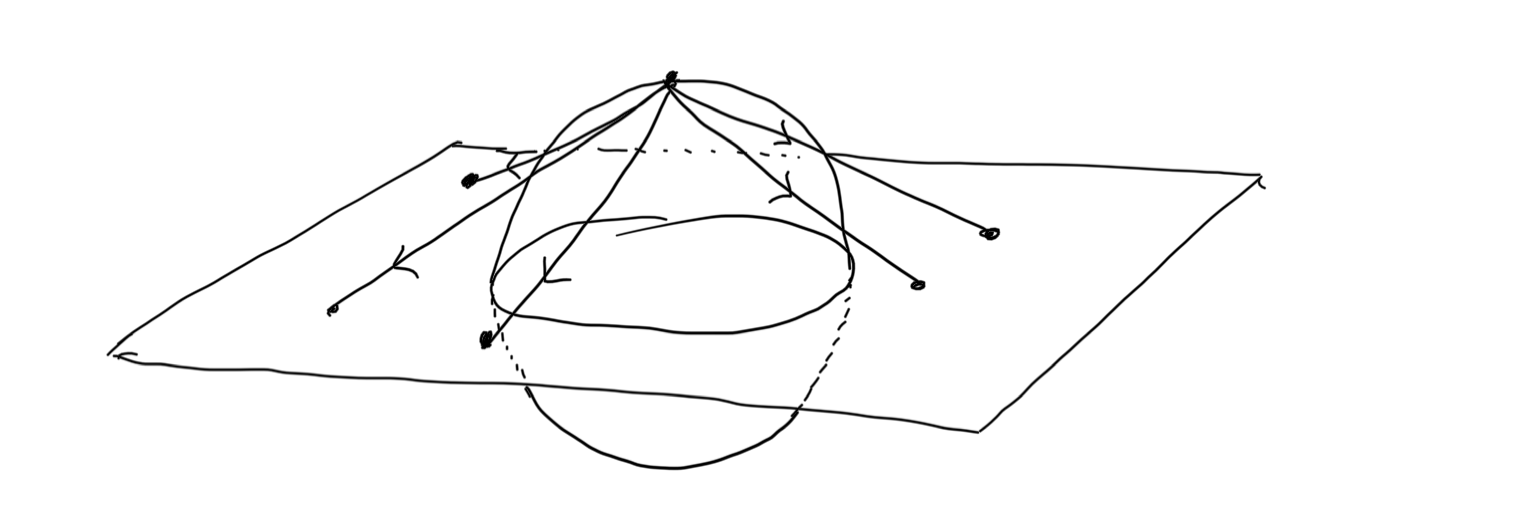
\includegraphics[scale=0.23]{img/Two_Dim_Stereographic_Projection.PNG}
    \end{center}
    \end{example}

    \begin{lemma}
    Let $X$ be a Hausdorff space. Then $X$ is locally compact at $x$ if and only if for every neighborhood $U$ of $x$, there is a neighborhood $V$ of $x$ such that $\bar{V}$ is compact and $\bar{V} \subset U$. 
    \end{lemma}

    \begin{corollary}
    Let $X$ be a locally compact Hausdorff space with $Y$ a subspace of $X$. If $Y$ is closed in $X$ or open in $X$, then $Y$ is locally compact. 
    \end{corollary}

    \begin{corollary}
    A space $X$ is homeomorphic to an open subset of a compact Hausdorff space if and only if $X$ is locally compact and Hausdorff. 
    \end{corollary}
